\documentclass[../SimBALink.tex]{subfiles}

\graphicspath{ {../Model/Powertrain/Motor_controller/Documentation/Figures/}{./Model/Powertrain/Motor_controller/Documentation/Figures/} }

\begin{document}

\subsection{Block diagram}
	\begin{figure}[h]
		\centering
		\includegraphics[width=\linewidth]{motor_controller_block_diagram}
		\caption{Motor controller - block diagram.}			\label{fig:motor_controller_block_diagram}
	\end{figure}
	\FloatBarrier

\subsection{Inputs and outputs}
	\subsubsection{Inputs}
	\begin{tabular}{ r | c | l | l }
		Signal						&	Symbol				&	MATLAB variable				&	Unit						\\\hline	
		Commanded motor current		&						&	\texttt{Motor\_Current\_Command}	&	\%					\\
		Commanded motor velocity		&						&	\texttt{Motor\_Velocity\_Command}	&	rpm			\\
		Commanded DC bus current		&						&	\texttt{Bus\_Current\_Command}	&	\%			\\
		Motor speed					&	$\omega_m$			&	\texttt{omega\_m}				&	rad/sec		\\
		Motor temperature				&	$T_m$				&	\texttt{T\_m}					&	\degree C		\\
		DC bus voltage				&	$V_\text{dc}$			&	\texttt{Vdc}					&	V
	\end{tabular}
	
	\subsubsection{Outputs}
		\begin{tabular}{ r | c | l | l }
			Signal						&	Symbol				&	MATLAB variable	&	Unit						\\\hline	
			Motor q-axis current			&	$I_q$				&	\texttt{Is.Iq}		&	rms amps			\\
			Motor d-axis current			&	$I_d$				&	\texttt{Is.Id}		&	rms amps
		\end{tabular}
	
\subsection{Background, rationale, modeling strategy}
	The motor controller model is actually two separate models: the motor controller, which makes control decisions based on rider commands and sensor feedback; and the power inverter, which is responsible for power conversion between DC and three-phase AC power.
	
	For this model, a simplified motor controller was developed based on documentation and working knowledge of the Tritium WaveSculptor 200, a commercially available unit used by the team. The power inverter was modeled as a lossless feedthrough pending the availability of efficiency data.
	
	\subsubsection{Motor control}
		A number of strategies for permanent-magnet synchronous motor (PMSM) control are available. Most modern strategies are based on space-vector control using the Park reference frame transformation. At their core, these strategies have the goal of determining the magnitude and phase of the motor current that should be used to achieve a given torque value.
		
		The WaveSculptor 200 uses so-called "$I_d = 0$" control, where the phase angle between the motor's back-emf and the motor phase current is controlled to zero. In the most common configuration, the the rider throttle input is mapped linearly to the motor torque command, which in turn is mapped linearly onto total motor current.
		
		\begin{equation}
			I_s =  \sqrt{ I_q^2 + I_d^2 } = I_{s,max} \times (\text{Rider throttle command})
		\end{equation}
		
		Since $I_d = 0$, the rider throttle input is effectively proportional to $I_q$. The model assumes that the motor controller has perfect control over stator currents.
		
		In addition to the throttle control loop, the WaveSculptor 200 implements five other control loops that can limit motor current:
		
		\begin{itemize}
			\item		Motor velocity
			\item		DC bus voltage
			\item		DC bus current
			\item		Power inverter temperature
			\item		Motor temperature
		\end{itemize}
		
		In the normal operation of the motor controller, each of these control loops runs simultaneously and generates a stator current command. A supervisory control loop chooses the smallest of all the current commands, and sends it to the inverter.
		
		\begin{figure}[h]
			\centering
			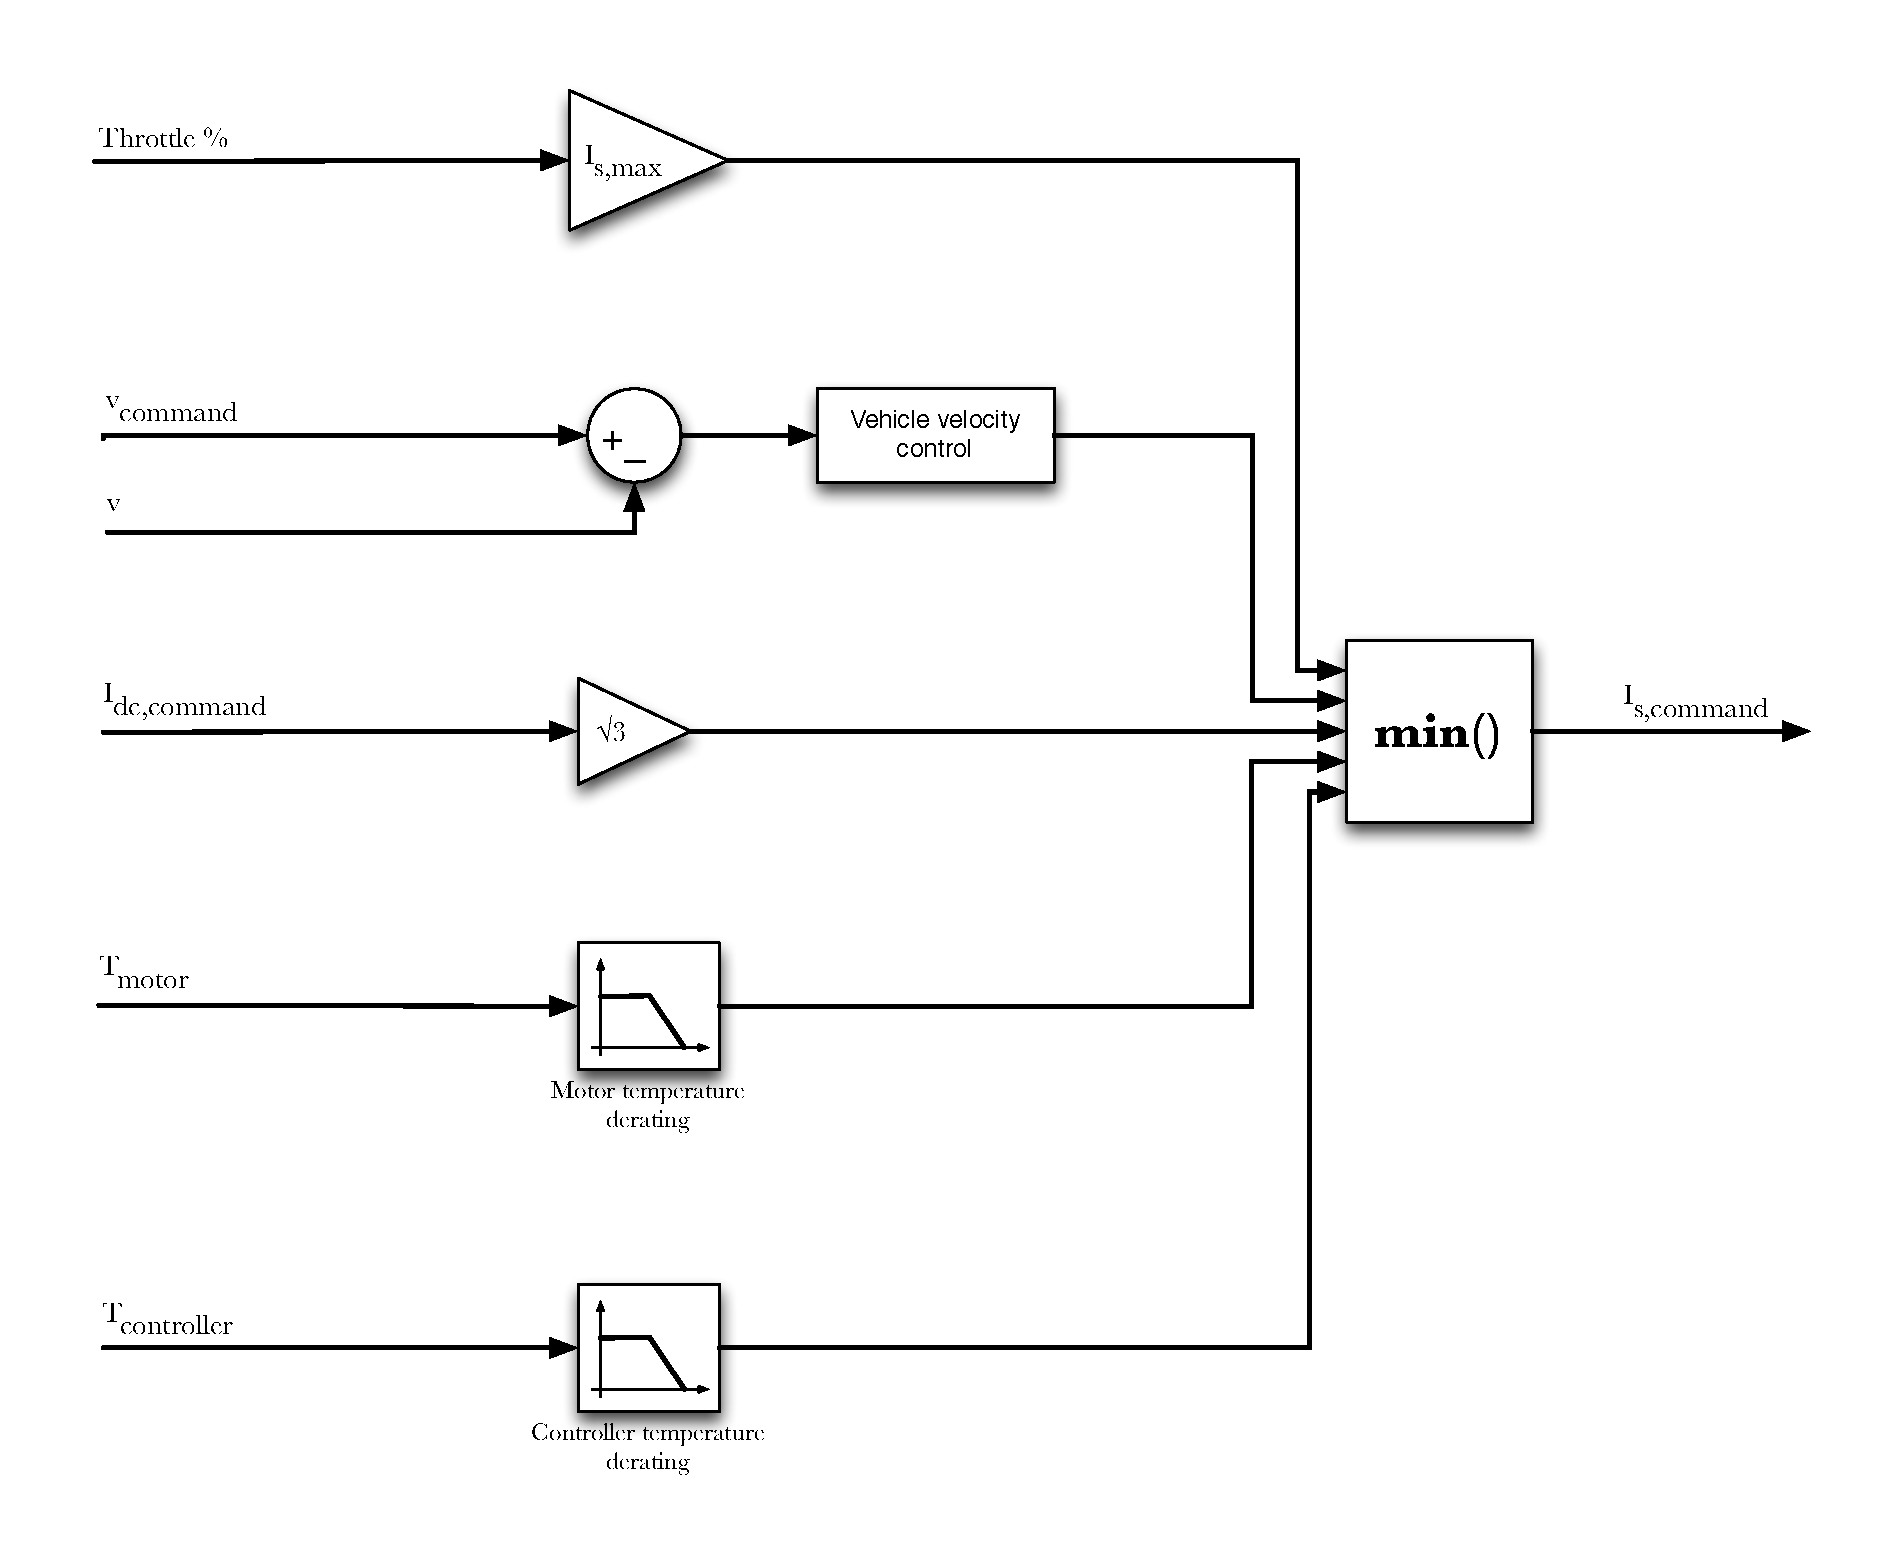
\includegraphics[width=\linewidth]{motor_controller_control_diagram}
			\caption{Motor control block diagram.}
			\label{fig:motor_controller_control_diagram}
		\end{figure}
		\FloatBarrier
		
		No calibration or validation data was available for most of the loops, and they do not typically affect motor controller operation. In this model, only the motor temperature and throttle command loops were implemented.
		
		\paragraph{Motor temperature derating}
			The motor temperature control loop affects the motor current by linearly derating the current once the motor temperature reaches a programmed value. Figure \ref{fig:motor_controller_temp_derating} shows the behavior of the motor temperature control loop.
			
			\begin{figure}[h]
				\centering
				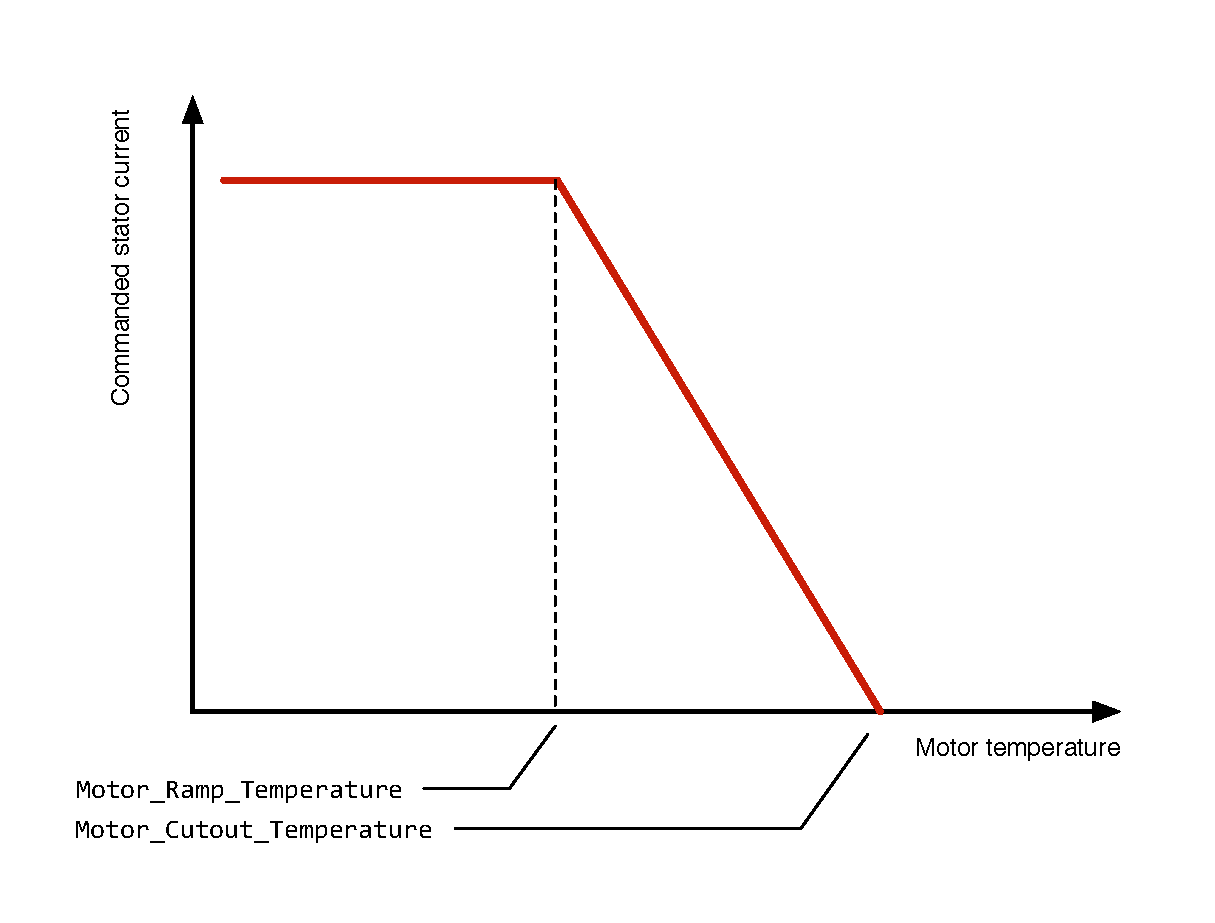
\includegraphics[width=\linewidth]{motor_controller_temp_derating}
				\caption{Motor temperature derating behavior.}
				\label{fig:motor_controller_temp_derating}
			\end{figure}
			\FloatBarrier
			
\subsection{Parameters}
	
	\renewcommand{\arraystretch}{1.5}
	\begin{tabular}{ p{5cm} | c | l | l }
		Parameter					&	Symbol				&	MATLAB variable						&	Unit						\\\hline	
		Maximum motor current			&	$I_{s,max}$			&	\texttt{Sine\_Current\_Limit}				&	rms amps					\\
		Motor temperature ramp point		&						&	\texttt{Motor\_Ramp\_Temperature}		&	\degree C						\\
		Motor temperature cutout point	&						&	\texttt{Motor\_Cutout\_Temperature}		&	\degree C			
	\end{tabular}


\subsection{Assumptions}
	\begin{itemize}
		\item 
			The power inverter is currently assumed to be lossless (this will be updated after better calibration data is obtained).
		\item
			The model assumes that the power inverter has perfect control over the phase currents. This assumption is valid over most of the operating range, but at high motor speeds especially, it may not be true. 
			
			Implementing a more accurate inverter model - specifically, a model that models switching dynamics - would improve the accuracy of the simulation, but this is a complex model operating on a time scale much slower than that of the overall simulation.
		\item
			The model currently assumes that the motor controller is cooled well enough that the inverter temperature will never limit operating performance.
			
	\end{itemize}

\end{document}